\documentclass[12pt,preprint]{aastex}
\usepackage[margin=1in]{geometry}
\usepackage{float,amsmath,bm,natbib,graphicx}
\citestyle{aa}

\defcitealias{ali_et_al2015}{A15}

\newcommand{\x}{\mathbf{x}}
\newcommand{\f}{\mathbf{f}}
\newcommand{\s}{\mathbf{s}}
\newcommand{\e}{\mathbf{e}}
\newcommand{\p}{\mathbf{p}}
\newcommand{\phat}{\widehat{\mathbf{p}}}
\newcommand{\C}{\mathbf{C}}
\newcommand{\Chat}{\mathbf{\widehat{C}}}
\newcommand{\F}{\mathbf{F}}
\newcommand{\Fhat}{\mathbf{\widehat{F}}}
\newcommand{\Q}{\mathbf{Q}}
\newcommand{\I}{\mathbf{I}}
\newcommand{\invC}{\ensuremath{\C^{-1}}}
\newcommand{\dC}[1]{\ensuremath{\C_{,#1}}}
\DeclareMathOperator{\Tr}{tr}
\newcommand{\half}{\ensuremath{\frac{1}{2}}}
\newcommand{\PDeriv}[2]{\ensuremath{\frac{\partial #1}{\partial #2}}}

\begin{document}

\title{Derivation and Application of the Jeffreys Prior \\for Estimating Signal Loss in PAPER} 
\author{Carina Cheng and the PAPER Collaboration}
\maketitle
\vspace{1cm}

The Jeffreys prior is an objective, non-informative prior distribution for a parameter space using Bayesian probability (\citealt{jaynes1968}). For the signal injection framework outlined in Cheng et al. (\textit{submitted}), we wish to compute the prior $p(P_{\rm in})$, or the probability density of the power spectrum of the EoR signal. 

The Jeffreys prior is defined as: 

\begin{equation}
\label{eq:jeffreys}
p(P_{\rm in}) \propto \sqrt {\Bigg\langle \Bigg(\frac{\partial \mathcal{L}}{\partial P_{\rm in}} \Bigg)^{2}\Bigg\rangle},
\end{equation}

\noindent where

\begin{equation}
\label{eq:logprob}
\mathcal{L} = \mathrm{ln} \, p(\widehat{P}_{\rm out} | P_{\rm in}),
\end{equation}

\noindent recalling that in our framework $P_{\rm in}$ is the power spectrum of the EoR signal (uniformly weighted), and $\widehat{P}_{\rm out}$ is the weighted output power spectrum of the data plus EoR.

For a single injection amplitude, our bootstrapped $\widehat{P}_{\rm out}$ values are well-approximated by a Gaussian distribution. Simplifying our notation so that $x = P_{\rm in}$ and $y = \widehat{P}_{\rm out}$:

\begin{equation}
\label{eq:prob}
p(y | x) = \frac{1}{\sigma(x) \sqrt{2\pi}} e^{-\frac{1}{2}\big(\frac{y-\bar y(x)}{\sigma}\big)^{2}},
\end{equation}

\noindent where $\sigma$ is the standard deviation of $\widehat{P}_{\rm out}$ and $\bar y$ is the mean of $\widehat{P}_{\rm out}$, and they are both functions of $P_{\rm in}$. Using Equations \eqref{eq:prob} and \eqref{eq:logprob}, the quantity inside the expectation value of Equation \eqref{eq:jeffreys} becomes:

%\begin{equation}
%\label{eq:logprob_full}
%\mathcal{L} = -\, log \, \sqrt{2\pi} - log\, \sigma - \frac{1}{2}\Big(\frac{y-\bar y}{\sigma}\Big)^{2}. 
%\end{equation}

%Next, the quantity inside the expectation value of Equation \eqref{eq:jeffreys} can be computed by taking the derivative of %Equation \eqref{eq:logprob_full} with respect to $P_{\rm in}$, or $x$:

\begin{eqnarray}
\Big(\frac{\partial \mathcal{L}}{\partial x} \Big)^{2} &=& \frac{1}{\sigma^{2}}\Big(\frac{\partial \sigma}{\partial x}\Big)^{2} -  \Big(\frac{2(y-\bar y)}{\sigma^{3}}\Big)\frac{\partial \sigma}{\partial x}\frac{\partial \bar y}{\partial x} - \Big(\frac{2(y-\bar y)^{2}}{\sigma^{4}}\Big)\Big(\frac{\partial \sigma}{\partial x}\Big)^{2} \nonumber \\
&+& \Big(\frac{(y-\bar y)^{2}}{\sigma^{4}}\Big)\Big(\frac{\partial \bar y}{\partial x}\Big)^{2} + \Big(\frac{2(y-\bar y)^{3}}{\sigma^{5}}\Big)\frac{\partial \sigma}{\partial x}\frac{\partial \bar y}{\partial x} + \Big(\frac{(y-\bar y)^{4}}{\sigma^{6}}\Big)\Big(\frac{\partial \sigma}{\partial x}\Big)^{2}.
\end{eqnarray}

Taking the expectation value then removes all terms with odd powers of $(y - \bar y)$ because those Gaussian moments evaluate to zero. Additionally, the second moment can be simplified since $\langle (y - \bar y)^{2} \rangle = \sigma^{2}$ and the fourth moment can be simplified since $\langle (y - \bar y)^{4} \rangle = 3\sigma^{4}$. Finally, after some additional simplification the Jeffreys prior becomes:

\begin{equation}
\label{eq:jeffreys_final}
p(x) \propto \sqrt{ \frac{1}{\sigma^{2}}\Big(2\Big(\frac{\partial \sigma}{\partial x}\Big)^{2} + \Big(\frac{\partial \bar y}{\partial x}\Big)^{2}\Big) }.
\end{equation}

When we simulate our full injection framework as in Cheng et al. (\textit{submitted}), we sample 50 $P_{\rm in}$ values that range from $\sim$ $10^{5}$\,mK$^{2}$ ($h^{-1}$ Mpc)$^{3}$ to $\sim$ 10$^{11}$\,mK$^{2}$ ($h^{-1}$ Mpc)$^{3}$, and we note that the prior is set to zero outside those regions. For the injections that we do sample, we can simply fit analytic functions to the mean and standard deviations of $\widehat{P}_{\rm out}$ ($\bar y$ and $\sigma$) as functions of $P_{\rm in}$. An example of the typical shape of these functions for the PAPER-64 analysis is shown in Figure \ref{fig:jeffreys1}, though in practice we fit solutions for every $k$-value and simulation independently.

\begin{figure}
	\centering
	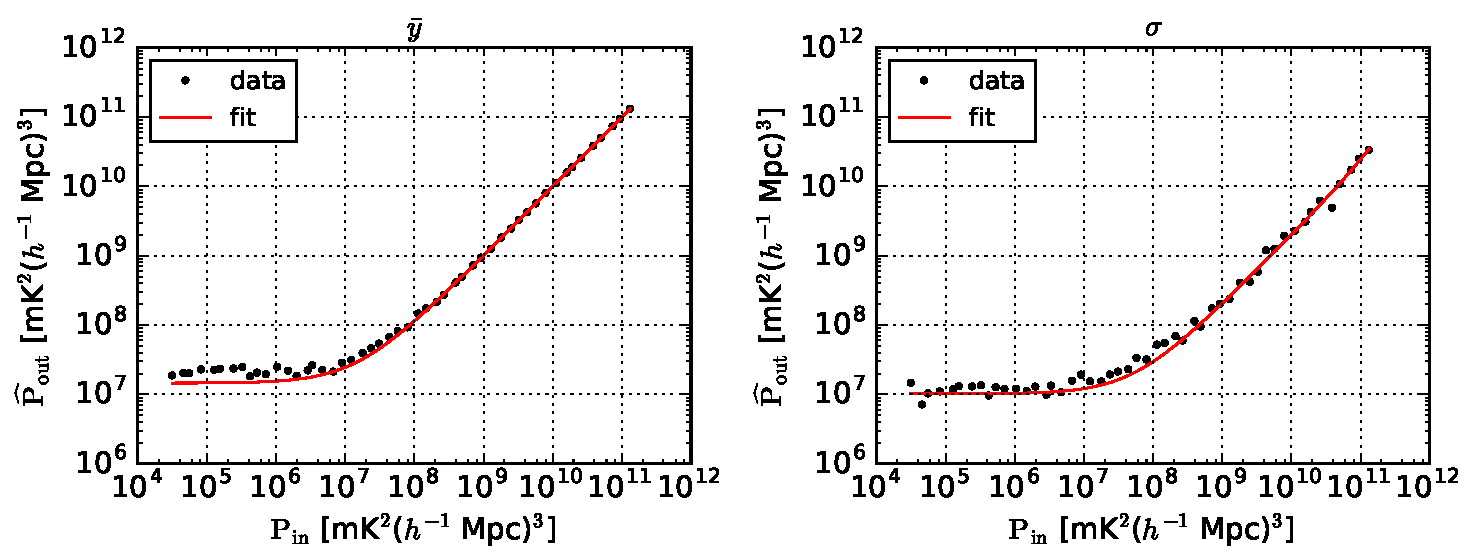
\includegraphics[width=\columnwidth]{plots/jeffrey_fits.pdf}
	\caption{An illustrative example (for the PAPER-64 analysis using uniform weighting and $k=0.393$\,$h$ Mpc$^{-1}$) of how the mean of $P_{\rm out}$ (left) and standard deviation of $P_{\rm out}$ (right) behave as a function of $P_{\rm in}$. Polynomials are fit to each (red) to describe how $\bar y$ and $\sigma$ evolve with $x$ (injection level), respectively, for the computation of the Jeffreys prior as defined in Equation \eqref{eq:jeffreys_final}. The polynomial fits for this example are $y = (-5.1 \times 10^{-15})x^{2} + x + (1.5 \times 10^{7})$ and $y = (5.0 \times 10^{-13})x^{2} + 0.2 x + 10^{7}$ for $\bar y$ and $\sigma$, respectively.}
	\label{fig:jeffreys1}
\end{figure}

We also show the typical shape of the Jeffreys prior used in our analysis in Figure \ref{fig:jeffreys2}, as computed by Equation \eqref{eq:jeffreys_final}. Most noticeably, it is not constant with $P_{\rm in}$, meaning a uniform prior, which is often used for simplicity, is informative in our application. Therefore, due to its objective nature we choose to use a Jeffreys prior in our analysis, multiplying our likelihood functions by Equation \eqref{eq:jeffreys_final} before computing posterior distributions.

\begin{figure}
	\centering
	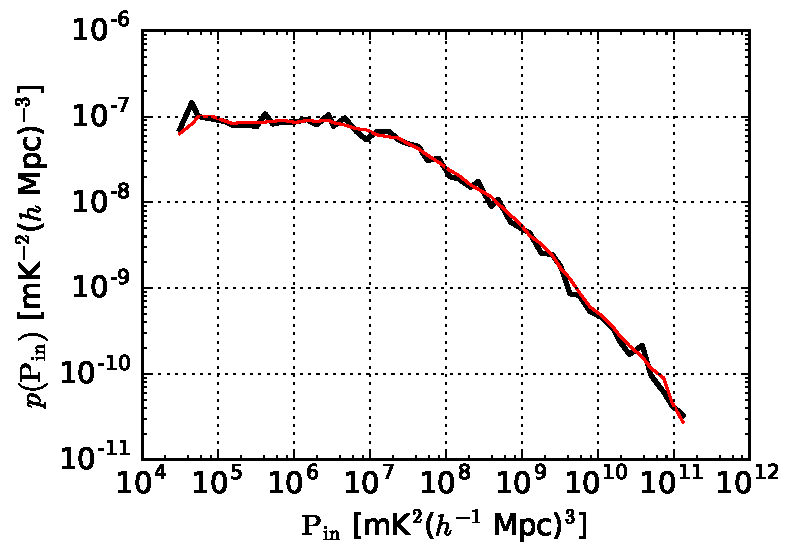
\includegraphics[width=10cm]{plots/jeffrey_prior.pdf}
	\caption{An example of the typical Jeffreys prior shape for the PAPER-64 analysis as computed by Equation \eqref{eq:jeffreys_final} (black). We smooth the prior using a sliding boxcar average over every $5$ injection levels (red). Most noticeably, the Jeffreys prior is not constant with $P_{\rm in}$, meaning a uniform prior would be an informative prior.}
	\label{fig:jeffreys2}
\end{figure}

\bibliographystyle{apj}
\bibliography{refs}


\end{document}
